\documentclass[11pt,a4paper]{article}

% ---------------------------------------------------------------------------
% Productive recovery and repeated harvesting in a reversible autocatalytic
% reactor: a uniform operating theorem with a machine-checked proof.
%
% Author metadata: set the macros below before submission.  They are
% deliberately left blank in this version.  \CompanionAuthor is the author
% printed for the companion manuscripts in refs.bib; \RepositoryNote is where
% the public repository location goes.
% ---------------------------------------------------------------------------
\newcommand{\PaperAuthor}{}
\newcommand{\PaperAffiliation}{}
\newcommand{\PaperDate}{15 September 2026}
\newcommand{\CompanionAuthor}{Anonymous}
\newcommand{\RepositoryNote}{The repository location will be supplied with the author information.}

\usepackage[T1]{fontenc}
\usepackage[utf8]{inputenc}
\usepackage{lmodern}
\usepackage{microtype}
\usepackage[a4paper,margin=1.05in]{geometry}
\usepackage{amsmath,amssymb,amsthm,mathtools}
\usepackage{booktabs}
\usepackage{array}
\usepackage{longtable}
\usepackage{enumitem}
\usepackage{xcolor}
\usepackage{graphicx}
\usepackage{tikz}
\usetikzlibrary{arrows.meta,positioning,calc}
\usepackage[obeyspaces,spaces]{url}
\usepackage[numbers,sort&compress]{natbib}
\usepackage[colorlinks=true,linkcolor=blue!55!black,citecolor=blue!55!black,urlcolor=blue!55!black]{hyperref}
\hypersetup{pdftitle={Productive recovery and repeated harvesting in a reversible autocatalytic reactor},
  pdfkeywords={autocatalysis, chemical reaction networks, serial transfer, impulsive differential equations, chemostat, template replication, Lean}}

\DeclareUrlCommand\lean{\urlstyle{tt}}
\setlist{itemsep=2pt,topsep=3pt}
\setlength{\emergencystretch}{1.5em}
\graphicspath{{figures/}}

\theoremstyle{plain}
\newtheorem{theorem}{Theorem}[section]
\newtheorem{proposition}[theorem]{Proposition}
\newtheorem{lemma}[theorem]{Lemma}
\newtheorem{corollary}[theorem]{Corollary}
\theoremstyle{definition}
\newtheorem{definition}[theorem]{Definition}
\theoremstyle{remark}
\newtheorem{remark}[theorem]{Remark}

\newcommand{\R}{\mathbb R}
\newcommand{\N}{\mathbb N}
\newcommand{\eps}{\varepsilon}
\newcommand{\dd}{\,\mathrm d}
\newcommand{\Adm}{\mathcal C}
\newcommand{\Bstar}{\mathcal B_*}
\newcommand{\Ent}{\mathcal E}
\newcommand{\Pulse}{\Pi}
\newcommand{\Flow}{\Phi}
\newcommand{\Pnet}{N}
\newcommand{\Iv}{I}

\title{Productive recovery and repeated harvesting\\ in a reversible autocatalytic reactor:\\[4pt]
\large a uniform operating theorem with a machine-checked proof}
\author{\PaperAuthor\\ \small \PaperAffiliation}
\date{\PaperDate}

\begin{document}
\maketitle

\begin{abstract}
Autocatalytic reaction structure does not by itself establish that a reactor can be harvested repeatedly. Withdrawal changes the chemical state, catalyst can be lost unequally across its bound and free forms, and replenishing food does not replace catalyst. We prove a uniform operating theorem for a specified, materially balanced, reversible mass-action source with fixed compatible thermochemistry: six reversible pairs on the species $U,W,X,C_1,C_2,Z$ with maintained fuel and waste, continuous food supply and washout, over a two-parameter rectangle of release and cleavage speeds. Each intervention withdraws $25$--$75\%$ of the well-mixed contents, permits up to $2\%$ additional species-dependent loss, and adds only food with a bounded refill error. A one-time conditioning period of twelve normalized time units carries any admitted preparation into an operating region; thereafter three units of recovery and one unit of collection return the actual chemical state to that region, for every admissible intervention and for interventions that depend on the current state. Every routine cycle exports at least $1/28$ template equivalents and at least $1/540$ of the free template species, while using at most $951/200$ of each food and at most $9/50$ gross fuel--waste service; the cumulative bounds for conditioning followed by $m$ cycles are explicit and linear in $m$. An inventory identity proves that the net covalent synthesis exceeds $m/28-11/10$, so production beyond any admitted initial stock is certified from the thirty-first cycle onward. The argument combines exact material relaxation, a growth inequality that holds only below a catalytic threshold, a strict exponential fence that replaces first-hitting-time constructions, and integrating-factor transfer inequalities between the catalytic phases. The trajectory, output, resource, arbitrary-finite-repetition and net-synthesis statements are verified in Lean~4 as one theorem; a conventional fixed-point argument adds a productive periodic hybrid trajectory for each fixed intervention. Targeted numerical experiments measure the conservatism of the certified constants. The result concerns a maintained schematic reactor; finite-copy reliability and molecular implementation are outside its scope and are delimited precisely.
\end{abstract}

\section{Introduction}\label{sec:intro}

Structural theories of autocatalysis, from Kauffman's autocatalytic sets~\citep{kauffman1986} through the RAF formalism~\citep{hordijk2004,steel2019} to the stoichiometric classification of autocatalytic cores~\citep{blokhuis2020}, certify that a reaction network can in principle regenerate its own catalysts from a food source. Experimental replicators~\citep{vonkiedrowski1986,lincoln2009,vaidya2012,ameta2021} and designed organic networks~\citep{semenov2016} show what such mechanisms look like chemically. The operational test that these experiments apply is older than any of the theory: since Spiegelman's serial-transfer experiments~\citep{mills1967}, a replicating system has been called self-sustaining when a fraction of a reaction mixture, diluted into fresh food, regrows to the point where the next transfer can be made, and this can be repeated indefinitely~\citep{lincoln2009}. The distinction between a system that replicates once and one that can be maintained through repeated dilution runs through the theory of replicators and reproducers~\citep{eigen1971,szathmary2006}, and questions about heredity and evolvability in autocatalytic networks~\citep{vasas2010} presuppose exactly such a maintenance protocol. The mathematical setting for that test is a hybrid dynamical system: a continuous flow between transfers and an instantaneous map at each transfer, as in impulsive differential equations~\citep{lakshmikantham1989}, superimposed on continuous-culture dynamics~\citep{smithwaltman1995}.

A companion paper~\citep{thermo2026} exhibits a thermochemically consistent chemical completion of a maintained autocatalytic exporter, six reversible pairs on eight species with a single standard-potential assignment across a rectangle of release and cleavage speeds, and transfers to it finite-copy operating certificates for fixed observation windows~\citep{exporter2026,finitecopy2026}. Those certificates concern a reactor that is prepared once and then observed. They say nothing about what happens after material is removed. A productive observation window is a weaker property than a repeatable harvesting operation, for three reasons. The withdrawal changes the state, and the post-withdrawal state need not belong to the class for which the observation-window theorem was proved. The catalyst exists in several chemical forms, free template and three bound phases, and species-dependent losses at the withdrawal step change their proportions. And the material returned to the reactor is food, which does not replace catalyst; the catalyst must be regrown by the reactor's own reactions before the next withdrawal. A repeatable theorem must therefore follow the disturbed state through its actual dynamics, prove that the endpoint again admits the next intervention, and bound output and supplies on that same trajectory.

This paper proves such a theorem for the deterministic mass-action concentration dynamics of the completed chemistry. The intervention class is broad: the retained fraction, the species-dependent loss factors and the food-refill errors range over intervals, and the intervention applied in cycle $n$ may depend arbitrarily on the state before that withdrawal. The source parameters are fixed throughout an operation but are arbitrary in their rectangle. No equilibrium approximation, no replacement of the disturbed state by a convenient preparation, and no independence between cycles enters the statement.

\paragraph{Contributions.}
\begin{enumerate}[label=(\roman*)]
\item \emph{A uniform operating theorem} (Theorem~\ref{thm:main}). From any admitted preparation, one conditioning pulse and twelve time units reach an operating region $\Bstar$. From $\Bstar$, every admissible pulse followed by three units of recovery returns the state to $\Bstar$, and the state stays there; the following unit is a collection window with certified output. The constants are explicit, the same for every parameter pair and every intervention sequence, and the theorem constructs the actual trajectories rather than assuming their existence.
\item \emph{Mechanism.} The two elemental totals relax exactly at unit rate, independently of every reaction. A weighted catalytic stock $Y$ grows at rate at least $2/3$ whenever it is at most $1/20$, because low stock forces the free foods to be abundant; globally positive drift is false and is not needed (Remark~\ref{rem:falsified}). A strict exponential fence with rate $3/5<2/3$ proves every scheduled deadline without constructing a first-hitting time (Lemma~\ref{lem:fence}). The threshold $1/20$ is not imposed by the chemistry: a first version of the theorem used $1/2500$, and raising it multiplied the certified window output by $125$ (Remark~\ref{rem:first}).
\item \emph{Free product.} Aggregate catalytic inventory is not free product. Integrating-factor comparisons along the actual phase-transfer reactions (Proposition~\ref{prop:transfer}) give $x(t+1/35)\ge Y(t)/27$ on the material corridor, hence a pointwise floor $1/540$ on the free template species throughout every collection window.
\item \emph{Net synthesis beyond the initial load} (Proposition~\ref{prop:synthesis}). An exact inventory identity, integrated across pulses and continuous segments and telescoped over cycles, proves that the integrated net covalent template synthesis exceeds $m/28-11/10$ after $m$ routine cycles. From the thirty-first cycle the certified production exceeds the largest admitted initial inventory.
\item \emph{Periodic operation and design rules.} For each fixed intervention the return map on the compact convex set $\Bstar$ is continuous, so Brouwer's theorem gives a productive four-unit periodic hybrid trajectory (Corollary~\ref{cor:periodic}). A retention design rule relates retained fraction, growth rate and sufficient recovery time (Proposition~\ref{prop:design}), and an exact entry-band calculation prepares a stochastic sequel (Proposition~\ref{prop:entry}).
\item \emph{Verification and diagnostics.} The trajectory, return, output, resource, repetition and net-synthesis statements are verified in Lean~4~\citep{demoura2021} with Mathlib~\citep{mathlib2020} as a single declaration (Appendix~\ref{app:formal}). Two hundred and twenty-four numerical segments measure how conservative the constants are (Section~\ref{sec:diagnostics}); an exact replay script re-derives every printed constant.
\end{enumerate}

\paragraph{Three kinds of evidence.}
Three kinds of statement appear and are kept apart. The source identities, the existence and uniqueness of nonnegative trajectories, the pulse image, the guarded growth and fence inequalities, the phase-transfer inequalities, the output, food and service integrals, arbitrary finite repetition and the net-synthesis bound are Lean-verified; Appendix~\ref{app:formal} maps each claim to a declaration. The general retention design rule, the compactness and continuity argument behind the periodic state, and the entry-band calculation are conventional proofs written out in full and labelled as such. The numerical experiments of Section~\ref{sec:diagnostics} are diagnostics: they show that the certified deadlines and floors are loose by moderate factors, and they prove nothing.

\paragraph{What is not claimed.}
The model is schematic chemistry with three formal elemental components, maintained fuel and waste activities, ideal mass action and one effective trimolecular reverse channel; no laboratory molecule is identified and no rate constant is fitted. The pulses are instantaneous and externally operated; handling time, control work and separation are not modelled, and the gross fuel--waste service counter measures a specified part of reactor operation, not the total work of the apparatus~\citep{rao2016}. The deterministic concentration equations are not a finite-copy law; nothing is asserted about the probability that a finite number of molecules survives a withdrawal, although Section~\ref{sec:discussion} states exactly what a finite-copy theorem must add. The periodic state is shown to exist, not to attract. The result assumes a preparation in the admitted region and provides no food-only startup protocol; the necessary initiation scale of~\citep{thermo2026} is the relevant statement for that question.

\paragraph{Organization.}
Section~\ref{sec:model} specifies the chemistry, the maintained flow, the interventions and the state regions. Section~\ref{sec:main} states the main theorem and discusses its quantifiers. Sections~\ref{sec:trajectories}--\ref{sec:output} prove it: trajectories, material relaxation and guarded growth (Section~\ref{sec:trajectories}); scheduled recovery (Section~\ref{sec:recovery}); output, free product and supplies (Section~\ref{sec:output}). Section~\ref{sec:repetition} assembles repetition, net synthesis and the periodic state. Section~\ref{sec:diagnostics} reports the numerical diagnostics, Section~\ref{sec:units} a dimensional reading, and Section~\ref{sec:discussion} the scope, the finite-copy sequel and open questions. Appendix~\ref{app:formal} contains the formal evidence and reproduction commands.

\section{The chemical source and the operating protocol}\label{sec:model}

\subsection{Reversible chemistry and common thermochemistry}\label{sec:chemistry}
The internal species are two foods $U,W$, the covalent template $X$, two substrate-binding complexes $C_1,C_2$ and a duplex $Z$. A fuel $F$ and a waste $P$ are maintained at unit activity. Write the concentration state as $c=(u,w,x,c_1,c_2,z)\in\R_{\ge0}^6$; concentrations and time are normalized. Put
\begin{equation}\label{eq:parameters}
\eps=\frac1{500\,000\,000},\qquad \eta=\frac1{8\,000\,000\,000},\qquad
19\le r\le21,\qquad \frac1{50}\le\delta\le\frac1{25}.
\end{equation}
The six reversible pairs and their net forward concentration fluxes are listed in Table~\ref{tab:pairs}. Pairs $1$--$4$ form the templated path $X+U+W\to C_1\to C_2\to Z\to 2X$, which is the autocatalytic completion; pair $0$ is basal, untemplated formation of $X$; pair $5$ is a driven cleavage of $X$ by the fuel, whose reverse is an effective trimolecular step and is not asserted to be elementary. The release speed $r$ and cleavage speed $\delta$ scale both directions of their pairs.

\begin{table}[tb]
\centering\small
\begin{tabular}{clll}
\toprule
Index & Reversible pair & Net forward flux & Role\\
\midrule
0 & $U+W\rightleftharpoons X$ & $j_0=\eps\,uw-(\eps/10)\,x$ & basal formation\\
1 & $X+U\rightleftharpoons C_1$ & $j_1=20\,xu-20\,c_1$ & substrate binding\\
2 & $C_1+W\rightleftharpoons C_2$ & $j_2=20\,c_1w-20\,c_2$ & substrate binding\\
3 & $C_2\rightleftharpoons Z$ & $j_3=20\,c_2-2\,z$ & templated ligation\\
4 & $Z\rightleftharpoons 2X$ & $j_4=r\,(z-x^2)$ & duplex release\\
5 & $X+F\rightleftharpoons U+W+P$ & $j_5=\delta\,x-\delta\eta\,uw$ & driven cleavage\\
\bottomrule
\end{tabular}
\caption{The six reversible pairs at unit fuel and waste activities. Each net flux is the forward mass-action rate minus the reverse one.}
\label{tab:pairs}
\end{table}

Assign three formal elemental units by
\[
\begin{gathered}
U=(1,0,0),\qquad W=(0,1,0),\qquad X=(1,1,0),\qquad C_1=(2,1,0),\\
C_2=Z=(2,2,0),\qquad F=P=(0,0,1),
\end{gathered}
\]
in the species order used throughout.
Every pair balances each unit. In units of thermal energy, one fixed vector of standard potentials is
\begin{equation}\label{eq:potential}
\mu^\circ=\bigl(0,\,0,\,-\log10,\,-\log10,\,-\log10,\,-2\log10,\,\log10+\log(8\cdot10^9),\,0\bigr)
\end{equation}
in the species order $U,W,X,C_1,C_2,Z,F,P$, and for each pair $\log(k_j^+/k_j^-)$ equals the reactant potential sum minus the product potential sum. This holds for every $(r,\delta)$ in~\eqref{eq:parameters}, because varying $r$ or $\delta$ changes both directions of its pair proportionally. The completion therefore uses one common thermochemistry rather than separately fitted equilibria, and the fuel--waste pair carries the affinity $\log(8\cdot10^{10})$ of the single emergent cycle in the sense of~\citep{polettini2014}. The realization and its count-level consequences are established in~\citep{thermo2026}; here only the concentration field is used, and its coefficients are bound to that realization (Appendix~\ref{app:formal}).

\subsection{Maintained flow and observables}\label{sec:flow}
Each internal species washes out at unit rate and each food enters at unit concentration rate. The concentration field is
\begin{equation}\label{eq:ode}
\begin{aligned}
u'&=1-u-j_0-j_1+j_5,&w'&=1-w-j_0-j_2+j_5,\\
x'&=-x+j_0-j_1+2j_4-j_5,&c_1'&=-c_1+j_1-j_2,\\
c_2'&=-c_2+j_2-j_3,&z'&=-z+j_3-j_4.
\end{aligned}
\end{equation}
Four linear observables organize the analysis: the two elemental totals, a weighted catalytic stock and the template inventory,
\begin{equation}\label{eq:observables}
\begin{aligned}
A&=u+x+2c_1+2c_2+2z,&B&=w+x+c_1+2c_2+2z,\\
Y&=x+\tfrac98c_1+\tfrac75c_2+\tfrac95z,&\Iv&=x+c_1+c_2+2z.
\end{aligned}
\end{equation}
$A$ and $B$ count the first and second elemental units among internal species. $\Iv$ counts template equivalents: one for each $X$, $C_1$ and $C_2$, two for the duplex. Under unit washout the effluent carries $\Iv$ template equivalents and $x$ free template per unit time, so the measured template-equivalent export on an interval is $\int\Iv\dd t$ and the free-$X$ export is $\int x\dd t$. Complexes contribute to $\Iv$ but not to free $X$. The weights of $Y$ are chosen so that its drift is favourable at low stock (Lemma~\ref{lem:growth}); $Y$ is a proof device, not a measured quantity. The gross fuel--waste service on $[a,b]$ is
\begin{equation}\label{eq:service}
G_{[a,b]}=\int_a^b\bigl(\delta x+\delta\eta\,uw\bigr)\dd t,
\end{equation}
counting both directions of the driven exchange without cancellation.

\begin{figure}[tb]
\centering
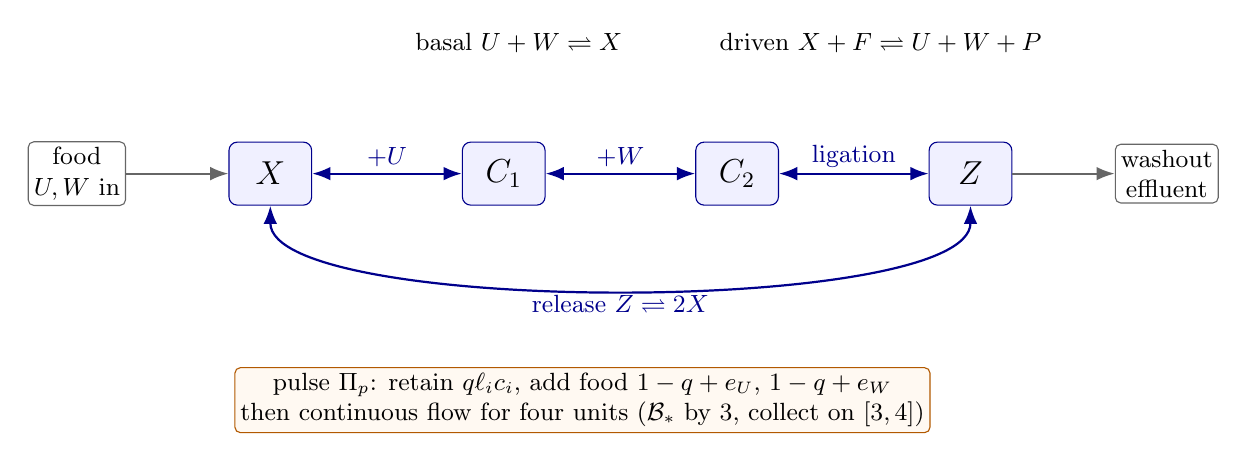
\begin{tikzpicture}[>=Latex,node distance=1.9cm,
  sp/.style={draw=blue!55!black,fill=blue!6,rounded corners=3pt,minimum width=1.05cm,minimum height=0.8cm,font=\large},
  lab/.style={font=\small},every node/.style={inner sep=2pt}]
\node[sp] (X) {$X$};
\node[sp,right=of X] (C1) {$C_1$};
\node[sp,right=of C1] (C2) {$C_2$};
\node[sp,right=of C2] (Z) {$Z$};
\draw[<->,thick,blue!55!black] (X) -- node[lab,above] {$+U$} (C1);
\draw[<->,thick,blue!55!black] (C1) -- node[lab,above] {$+W$} (C2);
\draw[<->,thick,blue!55!black] (C2) -- node[lab,above] {ligation} (Z);
\draw[<->,thick,blue!55!black] (Z.south) .. controls ($(Z.south)+(0,-1.4)$) and ($(X.south)+(0,-1.4)$) .. node[lab,below,pos=0.5] {release $Z\rightleftharpoons 2X$} (X.south);
\node[lab,above=1.05cm of C1.north,anchor=south west,xshift=-1.2cm] {basal $U+W\rightleftharpoons X$};
\node[lab,above=1.05cm of C2.north,anchor=south west,xshift=-0.3cm] {driven $X+F\rightleftharpoons U+W+P$};
\node[draw=black!60,rounded corners=2pt,left=1.3cm of X,align=center,font=\small] (food) {food\\$U,W$ in};
\draw[->,thick,black!60] (food) -- (X);
\node[draw=black!60,rounded corners=2pt,right=1.3cm of Z,align=center,font=\small] (out) {washout\\effluent};
\draw[->,thick,black!60] (Z) -- (out);
\node[below=2.05cm of C1.south,anchor=north,xshift=1.0cm,align=center,font=\small,draw=orange!70!black,rounded corners=2pt,fill=orange!5] (pulse)
 {pulse $\Pulse_p$: retain $q\ell_i c_i$, add food $1-q+e_U$, $1-q+e_W$\\ then continuous flow for four units ($\Bstar$ by $3$, collect on $[3,4]$)};
\end{tikzpicture}
\caption{Reaction pathways and external operation. All chemical links are reversible; the four-step templated path from $X+U+W$ to $2X$ is the autocatalytic completion. Continuous food input and washout act between instantaneous pulses. The full flux laws are in Table~\ref{tab:pairs}.}
\label{fig:network}
\end{figure}

\subsection{Interventions and state regions}\label{sec:pulse}
\begin{definition}[Admissible intervention]\label{def:pulse}
An intervention is $p=(q,\ell,e_U,e_W)$ with
\begin{equation}\label{eq:pulsebounds}
\frac14\le q\le\frac34,\qquad \frac{49}{50}\le\ell_i\le1\ \ (i=1,\dots,6),\qquad |e_U|,\ |e_W|\le\frac1{200}.
\end{equation}
Its pulse map $\Pulse_p:\R^6_{\ge0}\to\R^6_{\ge0}$ retains $q\ell_ic_i$ of every species and adds $1-q+e_U$ to $u$ and $1-q+e_W$ to $w$. The withdrawn state is $(1-q)c$, the additionally lost state is $q(1-\ell)c$, and refill adds no catalyst-bearing species. The pulse has zero modelled duration; the normalized reactor volume is restored externally.
\end{definition}
Here $q$ is the retained well-mixed fraction; $\ell_i$ allows up to $2\%$ further loss of each species, independently, for instance by adsorption or handling; $e_U,e_W$ are refill errors. Withdrawal and loss are external removals, not new reactions.

\begin{definition}[Admitted and operating regions]\label{def:regions}
\begin{align}
\Adm&=\{c\ge0:\ 9/10\le A(c),B(c)\le11/10,\ Y(c)\ge1/5000\},\label{eq:C}\\
\Bstar&=\{c\ge0:\ 159/160\le A(c),B(c)\le161/160,\ Y(c)\ge1/20\}.\label{eq:B}
\end{align}
\end{definition}
Both regions are nonempty and $\Bstar\subset\Adm$. For example, the state
\begin{equation}\label{eq:example}
(u,w,x,c_1,c_2,z)=(0.934,\,0.935,\,0.06,\,0.001,\,0.001,\,0.001)
\end{equation}
lies in $\Bstar$, with $A=B=1$ and $Y=0.064325$. The admitted region requires only that the elemental totals be within $10\%$ of their maintained values and that some catalyst be present; the operating region is much tighter in the material coordinates and asks for $250$ times more catalytic stock.

\begin{definition}[Operation]\label{def:operation}
Fix $(r,\delta)$ in~\eqref{eq:parameters}, an initial state $c\in\Adm$, a conditioning intervention $p_0$ and a protocol $\pi:\N\times\R^6_{\ge0}\to\{\text{admissible interventions}\}$. The conditioning trajectory $C$ solves~\eqref{eq:ode} from $C(0)=\Pulse_{p_0}(c)$ on $[0,12]$ and $s_0=C(12)$. For $n\ge0$ the routine trajectory $X_n$ solves~\eqref{eq:ode} from $X_n(0)=\Pulse_{\pi(n,s_n)}(s_n)$ on $[0,4]$, and $s_{n+1}=X_n(4)$. Cycle $n$ collects on $[3,4]$: $Q_n=\int_3^4\Iv(X_n)\dd t$ and $Q^{x}_n=\int_3^4x_n\dd t$. Its food use is $4+(1-q_n+e_{U,n})$ for $U$ and likewise for $W$; its service is $G_n=G_{[0,4]}(X_n)$. Conditioning uses $12+(1-q_0+e_{U,0})$ of $U$, similarly $W$, and service $G_{[0,12]}(C)$.
\end{definition}
The protocol may be an arbitrary function; no continuity or measurability is required. In cycle $n$ the intervention applied is $\pi(n,s_n)$, so it may respond to the pre-withdrawal state.

\section{The main theorem}\label{sec:main}

\begin{theorem}[Conditioning and repeatable harvesting]\label{thm:main}
Fix $(r,\delta)$ satisfying~\eqref{eq:parameters}, $c\in\Adm$, an admissible $p_0$ and any protocol $\pi$. Then the trajectories of Definition~\ref{def:operation} exist, are nonnegative, and are the unique nonnegative solutions from their post-pulse states, and:
\begin{enumerate}[label=(\alph*)]
\item\label{it:cond} (Conditioning) $C(t)\in\Bstar$ for every $t\ge12$; in particular $s_0\in\Bstar$.
\item\label{it:return} (Return) For every $n$: $Y(X_n(t))\ge1/20$ for all $t\ge5/2$, and $X_n(t)\in\Bstar$ for all $t\ge3$. In particular $s_{n+1}\in\Bstar$.
\item\label{it:output} (Output) For every $n$,
\begin{equation}\label{eq:output}
Q_n\ge\frac1{28},\qquad x_n(t)\ge\frac1{540}\ \text{ for all }t\in[3,4],\qquad Q^{x}_n\ge\frac1{540}.
\end{equation}
\item\label{it:supply} (Supplies) Each routine cycle uses at most $951/200$ of each food, including its pulse, and at most $9/50$ gross service. Conditioning uses at most $2551/200$ of each food and at most $27/50$ gross service.
\item\label{it:cumulative} (Repetition) For every integer $m\ge0$, conditioning followed by $m$ routine cycles satisfies, on these same concatenated trajectories,
\begin{equation}\label{eq:cumulative}
\sum_{n<m}Q_n\ge\frac m{28},\qquad
\text{food}_U,\ \text{food}_W\le\frac{2551+951m}{200},\qquad
G_{[0,12]}(C)+\sum_{n<m}G_n\le\frac{27+9m}{50}.
\end{equation}
\item\label{it:synthesis} (Net synthesis) Writing $\Pnet_m$ for the integral of $j_0+j_3-j_5$ over all continuous portions of conditioning and the first $m$ cycles,
\begin{equation}\label{eq:synthesis}
\Pnet_m\ge\frac m{28}-\frac{11}{10}.
\end{equation}
\end{enumerate}
\end{theorem}

\begin{remark}[Quantifiers and what the theorem constructs]
The parameter pair is fixed once and is otherwise arbitrary in its rectangle; the same constants hold at every corner. The intervention class is the full box~\eqref{eq:pulsebounds} at every cycle, and the protocol is arbitrary. The theorem is existential in the trajectories and universal in everything else: it constructs $C$ and every $X_n$ as global nonnegative solutions of the literal field, links each endpoint to the next starting state, and proves the bounds on those objects. The pulse withdrawals themselves and the continuous export outside the collection windows are excluded from $\sum Q_n$; counting them would only strengthen~\eqref{eq:synthesis}. Parts~\ref{it:cond}--\ref{it:synthesis} are compiled together as one Lean declaration whose statement is described in Appendix~\ref{app:formal}.
\end{remark}

\begin{remark}[The first compiled version and the threshold]\label{rem:first}
A first version of this theorem, also compiled, used the returned region $\{Y\ge1/2500,\ A,B\in[159/160,161/160]\}$, a four-unit recovery, collection on $[4,5]$ with $\int\Iv\ge1/3500$, food at most $1151/200$ and service at most $9/40$ per five-unit cycle. The strengthening to $\Bstar$ rests on one observation: the growth inequality of Lemma~\ref{lem:growth} holds up to $Y=1/20$ with the same free-food argument, not only up to $1/2500$. Nothing in the chemistry imposed the small guard. Raising it multiplies the certified window output by $125$ and improves the certified average export from $1/17500$ to $1/112$ per unit time, while shortening the cycle. No weight optimization, equilibrium search or attractor argument was involved; the constants of Section~\ref{sec:diagnostics} indicate that a further factor of about seven remains in the window output.
\end{remark}

\begin{remark}[Proof map]
Section~\ref{sec:trajectories} shows that nonnegative global trajectories exist and are unique, that $A$ and $B$ relax exactly to $1$, that the pulse image stays in the outer corridor $A,B\in[9/10,11/10]$ and retains at least $49/200$ of $Y$, and that $Y'\ge\tfrac23Y$ whenever $Y\le1/20$ in that corridor. Section~\ref{sec:recovery} turns the growth inequality into deadlines: $12$ for conditioning, $5/2$ for the routine catalytic target, $3$ for the material corridor. Section~\ref{sec:output} derives the output floors from $\Iv\ge\tfrac57Y$ and from phase transfer, and the supply bounds from the corridor. Section~\ref{sec:repetition} concatenates cycles and integrates the inventory identity.
\end{remark}

\section{Trajectories, material relaxation and guarded growth}\label{sec:trajectories}

\subsection{Global nonnegative trajectories}
\begin{lemma}[Material identities]\label{lem:material}
For every state and every $(r,\delta)$, the field~\eqref{eq:ode} satisfies
\begin{equation}\label{eq:materialid}
A'=1-A,\qquad B'=1-B,\qquad \Iv'=j_0+j_3-j_5-\Iv .
\end{equation}
Consequently, along any solution, $A(t)=1+(A(0)-1)e^{-t}$ and $B(t)=1+(B(0)-1)e^{-t}$.
\end{lemma}
\begin{proof}
Substitute~\eqref{eq:ode} into~\eqref{eq:observables}. In $A$ the coefficients of $j_0,\dots,j_5$ are $-1-1+1+2\cdot1-1+\dots$; carrying out the bookkeeping pair by pair, each reaction conserves the first elemental unit, so all fluxes cancel and only the inflow $1$ and the washout $-A$ remain. The same holds for $B$. In $\Iv$ the binding fluxes $j_1,j_2$ cancel ($C_1$ and $C_2$ each count one template equivalent, as does $X$), the release flux $j_4$ cancels ($Z$ counts two, $2X$ counts two), and $j_0$, $j_3$, $-j_5$ remain: basal formation creates one equivalent, ligation turns $C_2$ (one) into $Z$ (two), and cleavage destroys one. The scalar affine equations integrate explicitly.
\end{proof}

\begin{lemma}[Existence, nonnegativity and uniqueness]\label{lem:existence}
For $r,\delta\ge0$ and every $c\ge0$ there is a solution $X:[0,\infty)\to\R^6_{\ge0}$ of~\eqref{eq:ode} with $X(0)=c$. If $c$ is the pulse image of a state in $\Adm$, then any two nonnegative solutions from $c$ agree on $[0,\infty)$.
\end{lemma}
\begin{proof}
The field $f$ is polynomial, hence $C^1$. It is quasi-positive: if $c\ge0$ and $c_i=0$, every monomial in $f_i(c)$ with a negative sign contains the factor $c_i$ and vanishes, while the remaining terms are nonnegative; for $i\in\{u,w\}$ the inflow $1$ is present as well. Let $R=\max(A(c),B(c),1)$. Take a smooth bump $b:\R^6\to[0,1]$ equal to $1$ on the closed ball of radius $R$ and supported in the ball of radius $2R$, and let $\rho$ be the coordinatewise positive part, which is $1$-Lipschitz. The field $g=(b\,f)\circ\rho$ is bounded and globally Lipschitz, so the Picard--Lindel\"of theorem gives a global solution $X$ of $X'=g(X)$, $X(0)=c$. Each coordinate of $X$ stays nonnegative: at a point where $X_i=0$ the value $g_i(X)=b(\rho X)f_i(\rho X)$ is nonnegative by quasi-positivity, and a scalar barrier argument excludes a crossing of $0$. Hence $\rho X=X$ and $X'=b(X)f(X)$. By Lemma~\ref{lem:material}, $A(X)'=b(X)(1-A(X))$, which is $\le0$ whenever $A(X)\ge1$, so $A(X)\le\max(A(c),1)\le R$ by the upper barrier argument; likewise $B(X)\le R$. Every coordinate occurs in $A$ or $B$ with coefficient at least $1$, so $\|X(t)\|_\infty\le R$, $b(X(t))=1$, and $X$ solves the original field.

For uniqueness, both solutions start in the outer corridor $A,B\in[9/10,11/10]$ by Lemma~\ref{lem:pulse} below and stay there by Lemma~\ref{lem:material}; hence each coordinate is at most $11/10$ and both solutions remain in the closed ball of radius $2$. The polynomial field is Lipschitz on that compact convex ball, and the standard uniqueness theorem for ordinary differential equations applies on every $[0,t]$.
\end{proof}

The compact-support extension and the barrier arguments are the form in which the formal development constructs the trajectory; the mathematical content is the classical one~\citep{feinberg2019}: mass-action fields are quasi-positive, and the linear conservation-like relations of Lemma~\ref{lem:material} bound every coordinate.

\begin{lemma}[Material corridor and interior]\label{lem:corridor}
If a solution has $A(0),B(0)\in[9/10,11/10]$, then $A(t),B(t)\in[9/10,11/10]$ for all $t\ge0$ and $A(t),B(t)\in[159/160,161/160]$ for all $t\ge3$.
\end{lemma}
\begin{proof}
The corridor is immediate from the explicit formula. For the interior,
\[
e^3\ \ge\ 1+3+\frac{3^2}{2}+\frac{3^3}{6}+\frac{3^4}{24}=\frac{131}{8}>16,
\]
so $|A(t)-1|\le\tfrac1{10}e^{-t}<\tfrac1{160}$ for $t\ge3$.
\end{proof}

\subsection{The pulse image}
\begin{lemma}[Pulse image]\label{lem:pulse}
Let $c\ge0$ with $A(c),B(c)\in[9/10,11/10]$ and let $p$ be admissible. Then $c^+=\Pulse_p(c)\ge0$ and
\begin{equation}\label{eq:pulseimage}
\frac{1813}{2000}\le A(c^+),B(c^+)\le\frac{27}{25},\qquad
Y(c^+)\ge\alpha\,Y(c),\quad \alpha=\frac{49}{200},
\end{equation}
and each food pulse $1-q+e$ lies in $[49/200,151/200]$.
\end{lemma}
\begin{proof}
$A$ is linear with nonnegative coefficients and the food refill contributes exactly $1-q+e_U$ to $A$, so
\[
q\cdot\frac{49}{50}A(c)+1-q-\frac1{200}\ \le\ A(c^+)\ \le\ qA(c)+1-q+\frac1{200}.
\]
Both bounds are affine in $q$, so their extrema over the box are at corners: the minimum is attained at $q=3/4$, $A(c)=9/10$, giving $1813/2000$, and the maximum at $q=3/4$, $A(c)=11/10$, giving $27/25$. The same holds for $B$. Refill adds no catalyst-bearing species, so $Y(c^+)=\sum q\ell_i(\text{weight})_ic_i\ge q\cdot\tfrac{49}{50}Y(c)\ge\tfrac{49}{200}Y(c)$. The food bounds follow from~\eqref{eq:pulsebounds}.
\end{proof}
The pulse image is strictly inside the outer corridor $[9/10,11/10]$: the material state after a pulse is not reset to a preferred composition, but it is admitted by Lemma~\ref{lem:corridor}, which is all that the recovery argument needs.

\subsection{Guarded growth of the catalytic stock}
\begin{lemma}[Exact weighted drift and comparisons]\label{lem:drift}
For every state,
\begin{equation}\label{eq:drift}
Y'=(\eps+\delta\eta)\,uw+\Bigl(\tfrac52u-1-\delta-\tfrac\eps{10}\Bigr)x+\Bigl(\tfrac{11}{2}w-\tfrac{29}{8}\Bigr)c_1+\tfrac{11}{10}c_2+\Bigl(\tfrac r5-\tfrac{13}{5}\Bigr)z-\tfrac r5x^2 .
\end{equation}
For $c\ge0$, coefficient comparison gives
\begin{equation}\label{eq:comparisons}
A-u\le\tfrac{16}{9}Y,\qquad B-w\le\tfrac{10}{7}Y,\qquad x\le Y,\qquad \tfrac57Y\le\Iv\le A .
\end{equation}
\end{lemma}
\begin{proof}
Direct substitution; the comparisons hold coefficient by coefficient for nonnegative coordinates (the exact replay script checks each).
\end{proof}

\begin{lemma}[Parameterized surplus and guarded growth]\label{lem:growth}
Let $c\ge0$ with $A(c),B(c)\ge9/10$, let $\delta\le1/25$, $r\le21$, and let $Y(c)\le\beta$. Then
\begin{equation}\label{eq:surplus}
Y'-\tfrac23Y\ \ge\ (\eps+\delta\eta)\,uw+\Bigl(\tfrac{163}{300}-\tfrac1{5\cdot10^9}-\tfrac{389}{45}\beta\Bigr)x+\Bigl(\tfrac{23}{40}-\tfrac{55}{7}\beta\Bigr)c_1+\tfrac16c_2+\Bigl(\tfrac r5-\tfrac{19}5\Bigr)z .
\end{equation}
In particular, if also $r\ge19$ and $Y(c)\le1/20$, then $Y'\ge\tfrac23Y$.
\end{lemma}
\begin{proof}
By~\eqref{eq:comparisons}, $u\ge A-\tfrac{16}9Y\ge\tfrac9{10}-\tfrac{16}9\beta$ and $w\ge\tfrac9{10}-\tfrac{10}7\beta$, while $x^2\le\beta x$. Subtracting $\tfrac23Y$ from~\eqref{eq:drift} and substituting these bounds, $\delta\le1/25$ and $r\le21$ in the terms with negative sign gives~\eqref{eq:surplus}; explicitly, the difference between the two sides is
\[
\tfrac52\Bigl(u-\tfrac9{10}+\tfrac{16}9\beta\Bigr)x+\tfrac{11}2\Bigl(w-\tfrac9{10}+\tfrac{10}7\beta\Bigr)c_1+\Bigl(\tfrac1{25}-\delta\Bigr)x+\tfrac{21-r}5\beta x+\tfrac r5(\beta x-x^2),
\]
a sum of nonnegative terms. At $\beta=1/20$ the coefficients of $(x,c_1,c_2,z)$ in~\eqref{eq:surplus} are bounded below by
\[
\Bigl(\frac{4\,999\,999\,991}{45\,000\,000\,000},\ \frac{51}{280},\ \frac16,\ 0\Bigr),
\]
using $r\ge19$ for the last, and the food term is nonnegative. Hence the right side is nonnegative.
\end{proof}
The zero surplus in the $z$ coordinate is harmless: it means only that duplex alone does not grow $Y$ faster than rate $2/3$ at $r=19$; the inequality $Y'\ge\tfrac23Y$ is what is needed, and it is strict whenever any free or complexed template is present.

\begin{remark}[Globally positive drift is false]\label{rem:falsified}
The guard $Y\le1/20$ cannot be removed. At $c=(0,0,1,0,0,0)$ with $r=19$, $\delta=1/25$ one has $A=B=1$ but $Y'=-(1+\delta+\eps/10)-19/5<0$: high free template without food is consumed by washout, cleavage and dimerization faster than it is regenerated. This witness is compiled. The structure of the proof is therefore not a Lyapunov function or a global attractor, but a growth inequality on a sublevel set together with positive drift at its boundary; that is precisely what a scheduled recovery needs.
\end{remark}

\section{Scheduled recovery}\label{sec:recovery}

\subsection{A strict exponential fence}
The growth inequality is available only below the target, and the target has to be reached by a fixed deadline and kept afterwards. The direct route would construct the first time at which $Y$ reaches $\beta$ and argue separately before and after it. A single comparison avoids that.

\begin{lemma}[Strict fence]\label{lem:fence}
Let $\beta=1/20$. Let $y:[0,\infty)\to\R$ be differentiable with $y'=v$, let $b_0>0$ with $y(0)\ge b_0$, let $D\ge0$ satisfy $e^{(3/5)D}\ge\beta/b_0$, and suppose $v(t)\ge\tfrac23y(t)$ whenever $0\le y(t)\le\beta$. Then $y(T)\ge\beta$ for every $T\ge D$.
\end{lemma}
\begin{proof}
Fix $T\ge D$ and put $b(s)=\beta e^{(3/5)(s-T)}$ on $[0,T]$. Then $b'=\tfrac35b$, $b(T)=\beta$, $0<b\le\beta$ on $[0,T]$, and $b(0)=\beta e^{-(3/5)T}\le\beta e^{-(3/5)D}\le b_0\le y(0)$. Suppose $y$ touches $b$ from above at some $s\in[0,T]$, so $y(s)=b(s)\in(0,\beta]$. Then $v(s)\ge\tfrac23b(s)>\tfrac35b(s)=b'(s)$. A function that starts above a barrier and whose derivative strictly exceeds the barrier's derivative at every contact cannot cross below it; hence $y\ge b$ on $[0,T]$, and $y(T)\ge b(T)=\beta$.
\end{proof}
The fence rate $3/5$ is strictly below the source rate $2/3$ so that the contact inequality is strict, which is the hypothesis of the one-sided comparison theorem used; any rate in $(0,2/3)$ would do, with a correspondingly adjusted exponential bound. The lemma also proves persistence: once the deadline $D$ has passed, every later $T$ is covered by the same statement. Nothing is assumed about $y$ above $\beta$, which is essential in view of Remark~\ref{rem:falsified}.

\subsection{Deadlines}
\begin{proposition}[Conditioning and routine return]\label{prop:deadlines}
Let $X$ be the nonnegative solution from $\Pulse_p(c)$ with $p$ admissible.
\begin{enumerate}[label=(\alph*)]
\item If $c\in\Adm$, then $X(t)\in\Bstar$ for all $t\ge12$.
\item If $c\in\Bstar$, then $Y(X(t))\ge1/20$ for all $t\ge5/2$ and $X(t)\in\Bstar$ for all $t\ge3$.
\end{enumerate}
\end{proposition}
\begin{proof}
By Lemma~\ref{lem:pulse} the post-pulse state lies in the outer corridor, so by Lemma~\ref{lem:corridor} the whole trajectory does, and Lemma~\ref{lem:growth} gives $Y'\ge\tfrac23Y$ whenever $Y\le1/20$. Apply Lemma~\ref{lem:fence} to $y=Y(X(\cdot))$.

(a) $Y(c)\ge1/5000$, so $b_0=\tfrac{49}{200}\cdot\tfrac1{5000}=\tfrac{49}{10^6}$ and $\beta/b_0=50000/49$. The degree-nine Taylor polynomial gives
\[
e^{36/5}\ \ge\ \sum_{k=0}^{9}\frac{(36/5)^k}{k!}\ >\ \frac{50000}{49},
\]
so $D=12$ is admissible and $Y(X(t))\ge1/20$ for $t\ge12$. Lemma~\ref{lem:corridor} gives the inner material corridor for $t\ge3$.

(b) $Y(c)\ge1/20$, so $b_0=49/4000$ and $\beta/b_0=200/49$. Now
\[
e^{3/2}\ \ge\ 1+\frac32+\frac{(3/2)^2}{2}+\frac{(3/2)^3}{6}=\frac{67}{16}>\frac{200}{49},
\]
so $D=5/2$ is admissible: $Y(X(t))\ge1/20$ for $t\ge5/2$. Together with Lemma~\ref{lem:corridor}, $X(t)\in\Bstar$ for $t\ge3$.
\end{proof}
This proves parts~\ref{it:cond} and~\ref{it:return} of Theorem~\ref{thm:main}, given the concatenation of Section~\ref{sec:repetition}. Conditioning and routine recovery differ only in the starting stock: the one-time investment from $1/5000$ needs the long deadline, and its replenishment from $49/4000$ needs less than three units.

\begin{figure}[tb]
\centering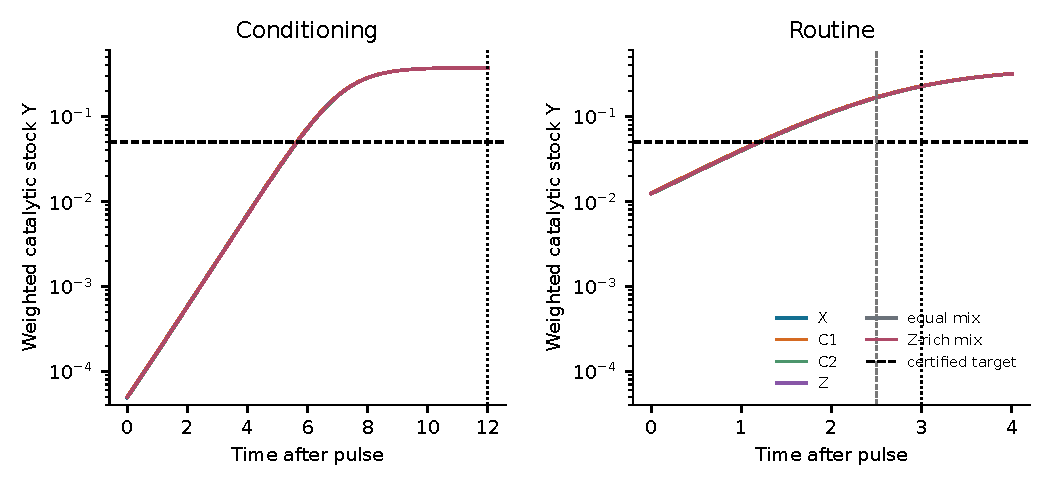
\includegraphics[width=\linewidth]{recovery.pdf}
\caption{Diagnostic recovery of the weighted catalytic stock $Y$ at $r=19$, $\delta=0.04$, $q=1/4$, adverse food error and species-dependent losses, for the four pure catalytic phases and two mixtures. Conditioning starts at $Y=1/5000$, $A=B=0.9$; routine trials start at $Y=1/20$, $A=B=159/160$, so the post-pulse stock is about $49/4000$. Horizontal lines mark the certified target $1/20$; vertical lines mark the certified deadlines ($12$ for conditioning, $5/2$ and $3$ for routine recovery). Curves are numerical solutions, not enclosures.}
\label{fig:recovery}
\end{figure}

\subsection{A retention design rule}
\begin{proposition}[Sufficient recovery allowance; conventional]\label{prop:design}
Suppose a pulse preserves at least $\alpha b_{\mathrm{init}}>0$ of the catalytic stock, that the material corridor is maintained, and that $Y'\ge\gamma Y$ whenever $Y\le\beta$. Then the catalytic target $\beta$ is reached by every $T$ with
\begin{equation}\label{eq:design}
T\ \ge\ T_{\mathrm{cat}}:=\max\Bigl\{0,\ \frac1\gamma\log\frac{\beta}{\alpha b_{\mathrm{init}}}\Bigr\}
\end{equation}
and is kept afterwards. The recovery deadline is $\max(T_{\mathrm{cat}},T_{\mathrm{mat}})$, where $T_{\mathrm{mat}}$ is the separate material deadline (here $3$).
\end{proposition}
\begin{proof}
Let $\tau$ be the first time at which $Y=\beta$, or $+\infty$. On $[0,\tau)$ the function $e^{-\gamma t}Y(t)$ is nondecreasing, so $Y(t)\ge\alpha b_{\mathrm{init}}e^{\gamma t}$ there; if $\tau$ exceeded $T_{\mathrm{cat}}$ this would give $Y(T_{\mathrm{cat}})\ge\beta$, a contradiction with continuity. After $\tau$, positive drift at the boundary $Y=\beta$ excludes a downward crossing.
\end{proof}
Equation~\eqref{eq:design} is sufficient, not necessary: the diagnostic hitting times of Section~\ref{sec:diagnostics} are well below it, and even a complete loss of inherited stock would leave the basal and reverse-driven initiation terms of~\eqref{eq:drift}, whose consequences are analysed in~\citep{thermo2026}. Figure~\ref{fig:retention} evaluates~\eqref{eq:design} across the retention interval with $\alpha=0.98q$, $\gamma=2/3$ and routine starting stock: at $q=1/4$ it gives about $2.10$, and the material deadline $3$ dominates throughout the interval. The rule separates the two things an operator can change, the retained fraction and the recovery time, from the one fixed by the chemistry, the rate $\gamma$.

\begin{figure}[tb]
\centering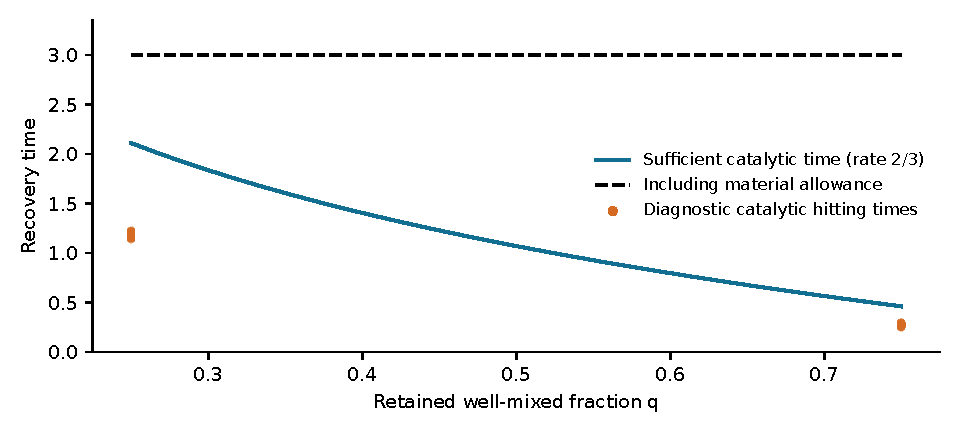
\includegraphics[width=0.9\linewidth]{retention.pdf}
\caption{Retention versus sufficient recovery time for routine starting stock, using~\eqref{eq:design} with $\alpha=0.98q$, $b_{\mathrm{init}}=\beta=1/20$ and $\gamma=2/3$. The three-unit material allowance dominates across the displayed interval. The points at the two tested retention values are diagnostic catalytic hitting times from Section~\ref{sec:diagnostics}; they are not a validated frontier and say nothing about intermediate retention values.}
\label{fig:retention}
\end{figure}

\section{Output, free product and supplies}\label{sec:output}

\subsection{Template-equivalent export}
By~\eqref{eq:comparisons}, $\Iv\ge\tfrac57Y$, and on the collection window $Y\ge1/20$ by Proposition~\ref{prop:deadlines}(b). Hence $\Iv\ge1/28$ on $[3,4]$ and $Q_n\ge1/28$, the first inequality of~\eqref{eq:output}. This is aggregate catalytic inventory in the effluent: free template together with its bound phases. A narrower observable requires transfer through the actual reactions.

\subsection{Phase transfer and the free-template floor}
\begin{lemma}[Phase comparison]\label{lem:phase}
Let $c\ge0$ with $A(c),B(c)\le11/10$, $19\le r\le21$ and $0\le\delta\le1/25$. Then the field~\eqref{eq:ode} satisfies
\begin{equation}\label{eq:phase}
x'\ge-70x+20c_1+38z,\qquad c_1'\ge-70c_1+20c_2,\qquad c_2'\ge-70c_2,\qquad z'\ge-70z+20c_2 .
\end{equation}
\end{lemma}
\begin{proof}
The corridor gives $u,w,x\le11/10$. In $x'=-x+j_0-j_1+2j_4-j_5$ the terms of negative sign are $-x$, $-(\eps/10)x$, $-20xu$, $-2rx^2$ and $-\delta x$; using $u\le11/10$, $x^2\le(11/10)x$, $r\le21$ and $\delta\le1/25$ their total coefficient is at most $1+\tfrac1{25}+\tfrac1{5\cdot10^9}+22+46.2<70$. The retained positive terms are $20c_1$ from $-j_1$ and $2rz\ge38z$ from $2j_4$; the remaining terms $\eps uw$ and $\delta\eta uw$ are nonnegative and are dropped. Similarly $c_1'\ge-(1+20+22)c_1+20c_2$, $c_2'\ge-(1+20+20)c_2$ and $z'\ge-(1+2+21)z+20c_2$, with loss coefficients $43,41,24\le70$.
\end{proof}

\begin{proposition}[Phase transfer]\label{prop:transfer}
Let $X$ be differentiable on $[0,\infty)$ with derivatives satisfying~\eqref{eq:phase} for all $t\ge0$. Then for every $h\ge0$,
\begin{equation}\label{eq:transfer}
x(h)\ \ge\ e^{-70h}\bigl[x(0)+20h\,c_1(0)+580h^2c_2(0)+38h\,z(0)\bigr].
\end{equation}
\end{proposition}
\begin{proof}
The tool is one comparison: if $g(0)\le f(0)$ and $g'(t)\le e^{70t}(f'(t)+70f(t))$ for $t\ge0$, then $g(t)\le e^{70t}f(t)$, because the right side is the derivative of $e^{70t}f$. Apply it four times. With $f=c_2$ and $g\equiv c_2(0)$, the inequality $c_2'\ge-70c_2$ gives $e^{70t}c_2(t)\ge c_2(0)$. With $f=c_1$ and $g(t)=c_1(0)+20t\,c_2(0)$: $e^{70t}(c_1'+70c_1)\ge20e^{70t}c_2\ge20c_2(0)=g'$, so $e^{70t}c_1(t)\ge c_1(0)+20t\,c_2(0)$; the same for $z$. Finally with $f=x$ and $g(t)=x(0)+20t\,c_1(0)+580t^2c_2(0)+38t\,z(0)$: $e^{70t}(x'+70x)\ge e^{70t}(20c_1+38z)\ge20c_1(0)+38z(0)+(400+760)t\,c_2(0)=g'(t)$, and $(400+760)/2=580$.
\end{proof}

\begin{corollary}[Free-template floor and export]\label{cor:freeX}
On a nonnegative trajectory in the outer material corridor, $x(t+1/35)\ge Y(t)/27$ for all $t\ge0$. Consequently, in every routine cycle, $x_n(t)\ge1/540$ for $t\in[3,4]$ and $Q^x_n\ge1/540$.
\end{corollary}
\begin{proof}
Shift time to $t$ and apply Proposition~\ref{prop:transfer} with $h=1/35$. The bracket is $x+\tfrac47c_1+\tfrac{116}{245}c_2+\tfrac{38}{35}z$; comparing with the weights $(1,\tfrac98,\tfrac75,\tfrac95)$ of $Y$, the smallest ratio is $\tfrac{116}{245}\big/\tfrac75=\tfrac{116}{343}$, so the bracket is at least $\tfrac{116}{343}Y(t)$. Since $e^2<9$ and $\tfrac{116}{343\cdot9}>\tfrac1{27}$, the floor follows. For $s\in[3,4]$ one has $s-\tfrac1{35}>\tfrac52$, so Proposition~\ref{prop:deadlines}(b) gives $Y(X_n(s-1/35))\ge1/20$ and hence $x_n(s)\ge1/540$; integrate over the unit window.
\end{proof}
The free-template floor is not an assumption that catalytic stock is free product: the actual reactions release $X$ from $C_1$ (dissociation), from $Z$ (release) and, through $C_1$, from $C_2$, and the polynomial coefficients of~\eqref{eq:transfer} are the minimal amounts that these reactions guarantee within the delay $1/35$. No matrix exponential or phase-by-phase numerical certificate is needed. The free-template floor is a factor $27\cdot\tfrac57\approx19$ below the aggregate floor because the aggregate bound does not pay for transfer.

\subsection{Food and service}
\begin{lemma}[Service and food budgets]\label{lem:supply}
On a nonnegative state with $A,B\le11/10$ and $\delta\le1/25$, the gross service rate satisfies $\delta x+\delta\eta uw<9/200$. Hence $G_{[0,4]}\le9/50$ and $G_{[0,12]}\le27/50$ along any corridor trajectory. Each food supply of a cycle is its elapsed time plus its pulse, so by Lemma~\ref{lem:pulse} a routine cycle uses at most $4+151/200=951/200$ of each food and conditioning at most $12+151/200=2551/200$.
\end{lemma}
\begin{proof}
$\delta x+\delta\eta uw\le\tfrac1{25}\cdot\tfrac{11}{10}+\tfrac1{25}\eta(\tfrac{11}{10})^2<\tfrac9{200}$; integrate.
\end{proof}
These are allowances on actual additions, including the refill error. The initial preparation and the withdrawn material are separate from them. This proves part~\ref{it:supply} of Theorem~\ref{thm:main}.

\section{Repetition, net synthesis and a periodic state}\label{sec:repetition}

\subsection{Existence of cycles and arbitrary repetition}
\begin{proposition}[One routine cycle]\label{prop:cycle}
For $c\in\Bstar$ and admissible $p$ there is a nonnegative solution $X$ from $\Pulse_p(c)$, unique by Lemma~\ref{lem:existence}, with $X(3),X(4)\in\Bstar$, $Q\ge1/28$, $x\ge1/540$ on $[3,4]$, $Q^x\ge1/540$, food at most $951/200$ each and service at most $9/50$. For $c\in\Adm$ there is likewise a conditioning trajectory with $C(12)\in\Bstar$, food at most $2551/200$ each and service at most $27/50$.
\end{proposition}
\begin{proof}
Lemma~\ref{lem:existence}, Proposition~\ref{prop:deadlines}, Section~\ref{sec:output}.
\end{proof}

\begin{theorem}[Arbitrary finite repetition]\label{thm:repeat}
For every protocol $\pi$ and every $s_0\in\Bstar$ there are states $(s_n)_{n\ge0}$ in $\Bstar$ and trajectories $(X_n)_{n\ge0}$ such that $X_n$ is the routine cycle of Proposition~\ref{prop:cycle} from $s_n$ with intervention $\pi(n,s_n)$ and $s_{n+1}=X_n(4)$; for every $m$ the sums of their outputs, foods and services satisfy the routine parts of~\eqref{eq:cumulative}.
\end{theorem}
\begin{proof}
Define $s_{n+1}$ recursively from $s_n$ by Proposition~\ref{prop:cycle}; the endpoint lies in $\Bstar$, so the recursion never leaves the hypothesis class. The cumulative bounds are the sums of the per-cycle bounds, by induction on $m$. Because the recursion uses only the existence statement, the protocol may depend on $s_n$ arbitrarily; no continuity, no measurability and no independence between cycles is involved. Uniqueness shows that the recursion is in fact determined by $s_0$ and $\pi$.
\end{proof}
Prefixing the conditioning trajectory gives parts~\ref{it:cond}, \ref{it:return}, \ref{it:output} and~\ref{it:cumulative} of Theorem~\ref{thm:main} in full.

\subsection{Net synthesis beyond the initial load}
An objection to any output bound is that the exported material might be inherited: an admitted preparation may contain up to $11/10$ template equivalents. The inventory identity settles this quantitatively.

\begin{lemma}[Integrated inventory balance]\label{lem:balance}
Let $X$ be a solution of~\eqref{eq:ode} on $[0,T]$ from $X(0)=\Pulse_p(c)$. Then
\begin{equation}\label{eq:fullbalance}
\Iv(X(T))-\Iv(c)+\int_0^T\Iv(X(t))\dd t+\Iv\bigl((1-q)c\bigr)+\Iv\bigl(q(1-\ell)c\bigr)
=\int_0^T(j_0+j_3-j_5)(X(t))\dd t .
\end{equation}
\end{lemma}
\begin{proof}
Integrate $\Iv'=j_0+j_3-j_5-\Iv$ from Lemma~\ref{lem:material} over $[0,T]$, and use $\Iv(\Pulse_p(c))=\Iv(c)-\Iv((1-q)c)-\Iv(q(1-\ell)c)$: the retained, withdrawn and lost parts of each coordinate sum to the coordinate, $\Iv$ is linear, and the food refill contributes nothing to $\Iv$.
\end{proof}
The right side is the net covalent synthesis of template equivalents on the segment: basal formation plus templated ligation minus driven cleavage. The left side accounts for every template equivalent that left the reactor as effluent, withdrawal or loss, plus the change in what remains.

\begin{proposition}[Net synthesis]\label{prop:synthesis}
In the operation of Theorem~\ref{thm:main}, $\Pnet_m\ge\sum_{n<m}Q_n-\Iv(c)\ge m/28-11/10$.
\end{proposition}
\begin{proof}
Apply~\eqref{eq:fullbalance} to the conditioning segment and to each routine segment. On each, the effluent integral, the withdrawn and the lost inventories are nonnegative, and on routine segment $n$ the effluent integral is at least $Q_n$. Hence $\Iv(s_0)-\Iv(c)\le\Pnet_{\mathrm{cond}}$ and $\Iv(s_{n+1})-\Iv(s_n)+Q_n\le\Pnet_n$. Summing telescopes the intermediate inventories: $\Iv(s_m)-\Iv(c)+\sum_{n<m}Q_n\le\Pnet_m$. Finally $\Iv(s_m)\ge0$ and, by~\eqref{eq:comparisons}, $\Iv(c)\le A(c)\le11/10$.
\end{proof}
This is part~\ref{it:synthesis} of Theorem~\ref{thm:main}. For $m\ge31$ the certified net synthesis is positive even against the largest admitted initial inventory, and the bound grows without limit with the number of cycles. The argument does not treat template equivalents as a conserved elemental quantity, which they are not: the elemental material arrives as food, and $\Iv$ is created and destroyed by the indicated reactions. It shows that the certified output cannot be explained by stock that was present at preparation.

\subsection{A productive periodic state}
\begin{corollary}[Periodic hybrid operation; conventional]\label{cor:periodic}
For each $(r,\delta)$ in~\eqref{eq:parameters} and each fixed admissible intervention $p$ there is a state $c_*\in\Bstar$ with $\Flow_4(\Pulse_p(c_*))=c_*$, where $\Flow_t$ is the flow of~\eqref{eq:ode}. The four-unit periodic hybrid trajectory obtained by repeating the pulse and the flow from $c_*$ has the output and resource guarantees of Theorem~\ref{thm:main} in every period, and its net synthesis per period equals exactly its effluent plus pulse and loss removals.
\end{corollary}
\begin{proof}
$\Bstar$ is the intersection of closed affine half-spaces with the nonnegative orthant, hence closed and convex; it is bounded because every coordinate is nonnegative and occurs in $A$ or $B$ with coefficient at least $1$; it is nonempty by the example after Definition~\ref{def:regions}; hence it is compact and convex. The return map $R(c)=\Flow_4(\Pulse_p(c))$ is well defined on $\Bstar$ by Lemma~\ref{lem:existence}. The pulse is affine. For initial states in its image all trajectories remain in the corridor $\|c\|_\infty\le11/10$, where the polynomial field has a uniform Lipschitz constant on a convex compact neighbourhood; Gronwall's inequality~\citep{gronwall1919} then gives continuous dependence at time $4$, so $R$ is continuous. Proposition~\ref{prop:deadlines}(b) gives $R(\Bstar)\subseteq\Bstar$. Brouwer's fixed-point theorem~\citep{granas2003} supplies $c_*$. At $c_*$ the endpoint difference in~\eqref{eq:fullbalance} vanishes.
\end{proof}
The corollary asserts existence. Neither uniqueness nor attraction of the periodic state follows, and the fixed intervention is essential: a discontinuous feedback protocol need not have a continuous return map, although Theorem~\ref{thm:repeat} still applies to it. This is the one part of the operating theory that is not Lean-verified, and it is not needed for Theorem~\ref{thm:main}.

\section{Numerical diagnostics}\label{sec:diagnostics}
The certified constants are uniform over the parameter rectangle, the intervention box and the regions; the experiments here ask how loose they are at specific corners. They were run with SciPy's Radau solver~\citep{hairer1996,virtanen2020} on the literal field~\eqref{eq:ode}, relative tolerance $10^{-9}$, absolute tolerance $10^{-12}$, with the effluent, free-template, service and net-synthesis integrals carried as additional coordinates and no clipping of any coordinate. The design was targeted, not exhaustive: all four parameter corners $(r,\delta)\in\{19,21\}\times\{0.02,0.04\}$; the four pure catalytic preparations (all of $Y$ in $X$, $C_1$, $C_2$ or $Z$) and two mixtures with $Y$-fractions $(\tfrac14,\tfrac14,\tfrac14,\tfrac14)$ and $(0.05,0.15,0.30,0.50)$; both retention endpoints $q\in\{1/4,3/4\}$; and two loss patterns, uniform $0.98$ and $(0.98,1,0.98,1,0.99,1)$. Food errors were adverse, $-0.005$. Conditioning trials started at $Y=1/5000$, $A=B=0.9$, and routine trials at $Y=1/20$, $A=B=159/160$: $96$ trials of each kind. For repeated intervention, eight cycles were run at each parameter corner from the explicit state in $\Bstar$, with retention cycling through $(0.25,0.75,0.4,0.6)$, alternating loss patterns and alternating refill error signs: $32$ cycles, each pulse acting on the actual preceding endpoint. Table~\ref{tab:diag} summarizes the $224$ continuous segments; the whole run took about $42$ seconds.

\begin{table}[tb]
\centering\small
\begin{tabular}{llll}
\toprule
Quantity & Certified & Observed range or extreme & Ratio\\
\midrule
Conditioning: time to reach $Y=1/20$ & $\le12$ & $4.656$ to $5.673$ & $2.1$\\
Conditioning: $Y$ at time $12$ & $\ge1/20$ & $0.375$ to $0.381$ & $7.5$\\
Conditioning: gross service on $[0,12]$ & $\le27/50$ & $\le0.0413$ & $13$\\
Routine: time to regain $Y=1/20$ & $\le5/2$ & $0.250$ to $1.226$ & $2.0$\\
Routine: $Y$ at time $4$ & $\ge1/20$ & $0.317$ to $0.364$ & $6.3$\\
Routine: template export on $[3,4]$ & $\ge1/28$ & $\ge0.2656$ & $7.4$\\
Routine: free-$X$ export on $[3,4]$ & $\ge1/540$ & $\ge0.1231$ & $66$\\
Routine: gross service on $[0,4]$ & $\le9/50$ & $\le0.0154$ & $12$\\
Repeated ($32$ cycles): template export & $\ge1/28$ & $\ge0.2854$ & $8.0$\\
Repeated ($32$ cycles): free-$X$ export & $\ge1/540$ & $\ge0.1332$ & $72$\\
Repeated: inventory residual~\eqref{eq:fullbalance} & $0$ & $\le5.8\cdot10^{-15}$ & \\
\bottomrule
\end{tabular}
\caption{Diagnostic summary of $192$ recovery trials and $32$ repeated cycles. The ratio column is the observed extreme divided by the certified bound (or the reverse for deadlines), rounded. Every trial satisfied every certified deadline, region and budget. The inventory residual is the linear identity~\eqref{eq:fullbalance} evaluated within the same solver run; it measures implementation consistency, not integration accuracy.}
\label{tab:diag}
\end{table}

Three readings are warranted. The deadlines are conservative by a factor of about two, and the output floors by seven to eight for template equivalents and by roughly seventy for free template; the free-template floor pays twice, for the aggregate bound and for the transfer delay. Both slowest recoveries were the pure-$C_2$ preparation at $r=19$, $\delta=0.04$, $q=1/4$ with uniform maximal loss, which is consistent with the zero $c_2$-to-$x$ direct link in~\eqref{eq:phase} and with $C_2$ having to pass through $Z$ or $C_1$ before releasing free template. The service budgets are loose by an order of magnitude because the corridor bound $x\le11/10$ is far above the free-template concentrations that actually occur. None of this is evidence for tighter uniform constants: the trials are $224$ points in a continuum of parameters, preparations and interventions, and the certified constants are supported by the inequalities of Sections~\ref{sec:trajectories}--\ref{sec:repetition} independently of them. Figure~\ref{fig:cycles} shows the repeated operation at one corner.

\begin{figure}[tb]
\centering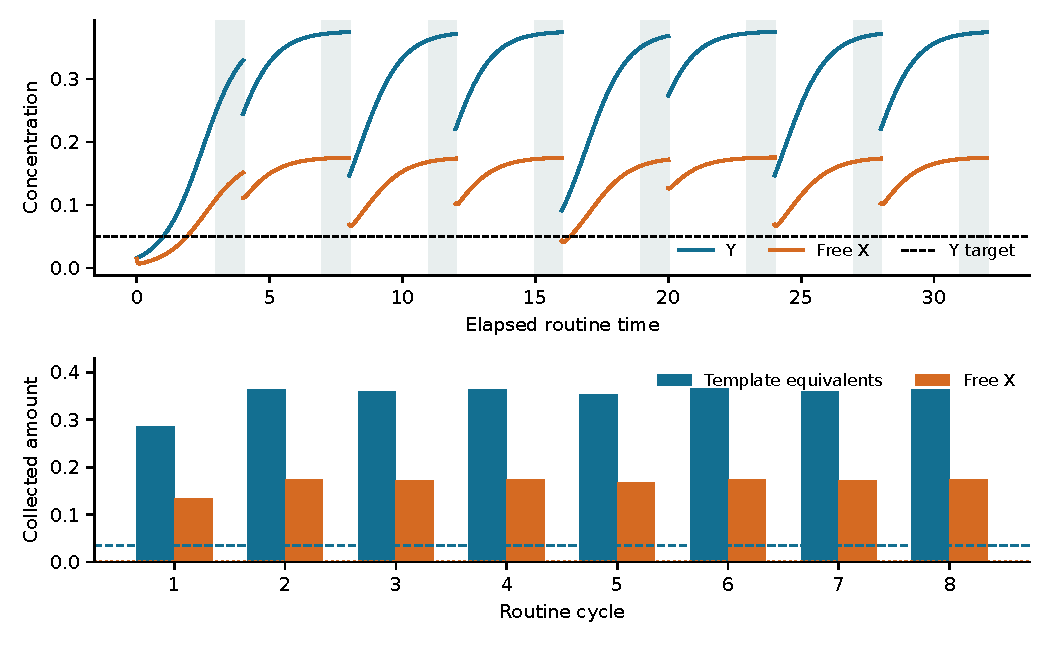
\includegraphics[width=\linewidth]{cycles.pdf}
\caption{Eight varying-intervention cycles at $r=19$, $\delta=0.04$, starting from the explicit state in $\Bstar$. Shaded intervals are collection windows. The lower panel compares collected template equivalents and free $X$ per cycle with their certified floors (horizontal lines). Each pulse acts on the actual preceding endpoint; retention, loss pattern and refill error vary from cycle to cycle.}
\label{fig:cycles}
\end{figure}

\section{A dimensional reading}\label{sec:units}
Take a concentration unit $c_*=1\,\mathrm{mM}$, a time unit $\tau_*=60\,\mathrm s$ and a reactor volume $V_R=1\,\mathrm{mL}$, so that one normalized amount is $V_Rc_*=1\,\mu\mathrm{mol}$. Theorem~\ref{thm:main} then reads as in Table~\ref{tab:units}. One-time conditioning lasts at most $12$ minutes and uses at most $12.755\,\mu\mathrm{mol}$ of each food and $0.540\,\mu\mathrm{mol}$ of gross fuel--waste service. These are in addition to the preparation, whose template inventory and elemental totals are each at most $1.1\,\mu\mathrm{mol}$ in their units.

\begin{table}[tb]
\centering\small
\begin{tabular}{ll}
\toprule
Routine quantity & Certified illustrative value\\
\midrule
Recovery / collection / cycle & $3\,\mathrm{min}$ / $1\,\mathrm{min}$ / $4\,\mathrm{min}$\\
Template-equivalent export per cycle & at least $35.71\,\mathrm{nmol}$\\
Free-$X$ export per cycle & at least $1.852\,\mathrm{nmol}$\\
Each food per cycle, including the pulse & at most $4.755\,\mu\mathrm{mol}$\\
Gross fuel--waste service per cycle & at most $0.180\,\mu\mathrm{mol}$\\
Certified net synthesis after $m$ cycles & at least $(m/28-1.1)\,\mu\mathrm{mol}$\\
\bottomrule
\end{tabular}
\caption{Illustrative dimensional values at $1\,\mathrm{mM}$, one minute and one millilitre. The numbers illustrate a unit conversion, not an experimental calibration.}
\label{tab:units}
\end{table}

For a reaction monomial of molecularity $m$ the consistent conversion is $k_{\mathrm{dim}}=k_{\mathrm{model}}/(\tau_*c_*^{m-1})$: the coefficient $20$ of a second-order binding step becomes about $333\,\mathrm{M^{-1}s^{-1}}$ and its first-order reverse becomes $1/3\,\mathrm{s^{-1}}$; the reservoir activities and their reference concentrations must be specified consistently when converting the full driven pair. Whether any laboratory chemistry has these coefficients is not a question this paper addresses.

\section{Scope, the finite-copy sequel and open questions}\label{sec:discussion}

\paragraph{What the theorem provides.}
A certified operating schedule for a balanced schematic chemistry, with two product observables of different strength, explicit resource allowances, arbitrary repetition under state-dependent interventions, and a proof that the exported material is synthesized rather than inherited. In the language of serial-transfer experiments~\citep{mills1967,lincoln2009}, the theorem states the transfer fraction, the recovery time and the yield for which the system is self-sustaining, and it does so uniformly over a box of transfer conditions rather than for one protocol. In the language of continuous culture~\citep{smithwaltman1995}, it is a return theorem for a pulsed chemostat with a hybrid pulse map~\citep{lakshmikantham1989}, proved by scalar comparison rather than by a global Lyapunov function; Remark~\ref{rem:falsified} explains why the latter is unavailable.

\paragraph{What it does not provide.}
Molecular identities, measured rate constants, biological functionality and purification are not established; free $X$ in the effluent is a narrower observable than aggregate inventory but is still mixed effluent, and a practical implementation would have to realize the effective reverse trimolecular channel. Maintained fuel and waste activities are part of the external operation, and a finite integrated service allowance does not by itself show that a finite autonomous reservoir can keep those activities constant; the activity-corridor relation of~\citep{thermo2026} states what a finite bath would additionally require. Instantaneous pulses omit handling time, and gross chemical service is not the total work of solvent exchange, pumping, control or separation; the open-network balances of~\citep{rao2016,polettini2014} are the framework in which those distinctions are kept.

\paragraph{The finite-copy question.}
The deterministic equations are the large-volume limit of a count process~\citep{kurtz1972,anderson2015}; the companion count model uses the falling factorial $N_X(N_X-1)$ for the identical-reactant pair $2X\rightleftharpoons Z$, whereas~\eqref{eq:ode} uses $x^2$, and its canonical export marks are four times the template-equivalent observable used here. A finite-copy version of Theorem~\ref{thm:main} must specify the withdrawal kernel at the level of molecules, including species losses and refill rounding; bound the post-pulse catalytic and material lower tails conditionally on the actual pre-pulse state; prove return, output and service on one continued count law, with free-template export counted as free-$X$ washout events; and iterate a conditional one-cycle bound, so that a uniform conditional failure probability $\epsilon$ after any successful past gives $m$-cycle success at least $(1-\epsilon)^m$ without an independence assumption. The present theorem supplies the nested regions, the retained-stock margin, the growth inequality and the budgets that such a proof consumes; companion analyses of finite-count inheritance under bounded food~\citep{inheritance2026} and of permanence and composition control under a dynamic reservoir~\citep{permanence2026} treat related questions on different sources and are not prerequisites here. One exact calculation is worth recording, because a stochastic entry event needs a target with interior margin.

\begin{proposition}[Entry band; conventional]\label{prop:entry}
Let $\Ent=\{c\ge0:\ 79/80\le A,B\le81/80,\ Y\ge9/200\}$. Then $\Bstar\subset\Ent$ with material margin $1/160$ and catalytic margin $1/200$, and every admissible pulse from a state in $\Ent$, followed by the flow, gives $Y\ge1/20$ for all $t\ge8/3$, a state in $\Bstar$ for all $t\ge3$, and the free-template floor $1/540$ on $[3,4]$.
\end{proposition}
\begin{proof}
$\Ent$ lies in the outer corridor, so Lemmas~\ref{lem:pulse}, \ref{lem:corridor} and~\ref{lem:growth} apply; the retained stock is at least $\tfrac{49}{200}\cdot\tfrac9{200}=\tfrac{441}{40000}$ and $\beta/b_0=2000/441$. Now $e^{8/5}\ge1+\tfrac85+\tfrac{(8/5)^2}2+\tfrac{(8/5)^3}6=\tfrac{1711}{375}>\tfrac{2000}{441}$, so Lemma~\ref{lem:fence} with $D=8/3$ gives the catalytic statement; Lemma~\ref{lem:corridor} gives $\Bstar$ by $3$; and $\tfrac83+\tfrac1{35}<3$ makes Corollary~\ref{cor:freeX} available on $[3,4]$.
\end{proof}
No finite-copy probability is asserted here, and none follows from the deterministic diagnostics of Section~\ref{sec:diagnostics}.

\paragraph{Open questions.}
Four seem most natural. First, the optimal deadlines: the diagnostics suggest that recovery could be certified in about half the time, which would require a growth inequality with a state-dependent rate or a two-stage fence. Second, attraction: whether the periodic state of Corollary~\ref{cor:periodic} is unique and attracting on $\Bstar$, which the present comparison methods do not address. Third, feedback: whether a state-dependent protocol can be chosen to maximize certified yield per unit of food or service, a control problem on the hybrid system. Fourth, robustness to parameter changes that do not preserve the equilibrium ratios; the present result covers only the thermochemically consistent rectangle, by design.

\paragraph{Data and code availability.}
\RepositoryNote{} The Lean sources, the verification receipts, the numerical script and its output, the figure script and an exact replay script for every printed constant accompany the manuscript source.

\appendix
\section{Formal evidence and reproduction}\label{app:formal}
The frozen environment is Lean~4 (toolchain \lean{leanprover/lean4:v4.30.0}) with the repository's pinned Mathlib manifest. Verification treats compiler warnings as errors, exports declaration types and reports the axioms used. The central theorem is
\begin{center}\lean{ProductiveRecovery.conditioned_productive_operation}\end{center}
in the module \lean{proofs/ProductiveRecovery/PostproofResolution.lean}. Its hypotheses are real parameters $r\in[19,21]$, $d\in[1/50,1/25]$, a conditioning intervention, a protocol \lean{protocol : Nat -> State -> Intervention} and an admitted state. Its conclusion is the existence of a conditioning trajectory $C$, a state sequence $s$ and routine trajectories $X_n$ such that: $C(0)$ is the pulse image; $C$ is nonnegative and satisfies the derivative equation of the literal field at every $t\ge0$; $s_0=C(12)$ and every $s_n$ lies in $\Bstar$; each $X_n$ starts at the pulse image of $s_n$ under \lean{protocol n (s n)}, ends at $s_{n+1}=X_n(4)$, is nonnegative, satisfies the derivative equation, lies in $\Bstar$ at times $3$ and $4$, has $x_n\ge1/540$ on $[3,4]$ and $\int_3^4x_n\ge1/540$; and for every $m$ the cumulative template output, both food totals, the total service and the net synthesis satisfy~\eqref{eq:cumulative}--\eqref{eq:synthesis}. The strict receipt records exit code $0$, empty compiler output, $36$ current dependency sources and artifacts, five exported declaration interfaces and $106$ seconds of verification time. The formal evidence uses only the ordinary axioms \lean{propext}, \lean{Classical.choice} and \lean{Quot.sound}; there are no admitted placeholders, no native numerical certificates and no warning suppression in the theorem chain. The compiled statement quantifies over the interventions through the structure \lean{Intervention}, whose fields carry the bounds~\eqref{eq:pulsebounds} as proof obligations.

\begin{longtable}{>{\raggedright\arraybackslash}p{0.36\linewidth}>{\raggedright\arraybackslash}p{0.58\linewidth}}
\toprule Claim & Declaration (namespace \lean{ProductiveRecovery} unless stated)\\\midrule\endhead
\bottomrule\endlastfoot
Literal stoichiometry and coefficient binding to the realization & \lean{field_stoichiometry}; \lean{flux_coefficients}; \lean{CommonPhysicalRealization.material_balance}, \lean{CommonPhysicalRealization.common_thermochemistry}~\citep{thermo2026}\\
Material and inventory identities, exact drift (Lemmas~\ref{lem:material}, \ref{lem:drift}) & \lean{material_A}; \lean{material_B}; \lean{inventory_drift}; \lean{weighted_drift}; \lean{material_to_food}; \lean{inventory_lower}\\
Global nonnegative trajectories (Lemma~\ref{lem:existence}) & \lean{boundary_nonneg}; \lean{extension_solution}; \lean{global_nonnegative_solution}\\
Uniqueness for admitted pulse trajectories & \lean{corridor_norm}; \lean{bounded_source_unique}; \lean{actual_return_unique}\\
Exact material solution, corridor and interior (Lemma~\ref{lem:corridor}) & \lean{affine_material_solution}; \lean{scalar_material_corridor}; \lean{strong_material_interior}\\
Pulse image and retention (Lemma~\ref{lem:pulse}) & \lean{pulse_nonnegative}; \lean{pulse_material}; \lean{pulse_catalyst}; \lean{food_feasible}; \lean{removal_accounting}\\
Parameterized surplus and guarded growth (Lemma~\ref{lem:growth}) & \lean{parameterized_drift}; \lean{strong_guarded_growth}; earlier guard \lean{guarded_growth}\\
Global positive drift is false (Remark~\ref{rem:falsified}) & \lean{global_positive_drift_false}\\
Strict fence (Lemma~\ref{lem:fence}) & \lean{strong_scheduled_recovery}; earlier \lean{guarded_scheduled_recovery}, \lean{recovered_floor_invariant}\\
Conditioning and routine return (Proposition~\ref{prop:deadlines}) & \lean{strong_trajectory_return}; \lean{conditioning_return}; \lean{routine_return}\\
Phase comparison and transfer (Lemma~\ref{lem:phase}, Proposition~\ref{prop:transfer}) & \lean{phase_comparison}; \lean{factor_comparison}; \lean{phase_transfer}\\
Free-template floor and export (Corollary~\ref{cor:freeX}) & \lean{free_phase_floor}; \lean{routine_free_export}\\
Service and food budgets (Lemma~\ref{lem:supply}) & \lean{gross_service_bound}; \lean{service_over_bound}; \lean{routine_output_supplies}\\
One routine cycle and conditioning (Proposition~\ref{prop:cycle}) & \lean{exists_routine_cycle}; \lean{exists_conditioning}\\
Arbitrary repetition (Theorem~\ref{thm:repeat}) & \lean{RoutineCycle}; \lean{routineStates}; \lean{arbitrary_routine_operation}\\
Integrated inventory balance (Lemma~\ref{lem:balance}) & \lean{inventory_balance_over}; \lean{pulse_balance_over}; \lean{full_cycle_inventory_balance}\\
Net synthesis (Proposition~\ref{prop:synthesis}) & \lean{net_over_lower}; \lean{routine_net_lower}; \lean{synthesis_telescoping}; \lean{inventory_initial_bound}\\
Theorem~\ref{thm:main}, all parts & \lean{conditioned_productive_operation}\\
First compiled version (Remark~\ref{rem:first}) & \lean{productive_recovery}; \lean{arbitrary_finite_operation}\\
Design rule (Proposition~\ref{prop:design}), periodic state (Corollary~\ref{cor:periodic}), entry band (Proposition~\ref{prop:entry}) & conventional proofs in the text; the fixed-target fence they rely on is \lean{strong_scheduled_recovery}\\
\end{longtable}

The realization paper's count source assigns export marks $4,4,4,8$ to washout of $X,C_1,C_2,Z$; dividing by four gives the template-equivalent observable $\Iv$ used here. Its identical-reactant reverse propensity uses $N_X(N_X-1)$ where~\eqref{eq:ode} uses $x^2$. The coefficient binding authenticates the concentration field and its coefficients against that realization; it does not identify a finite-count trajectory with the solution of~\eqref{eq:ode}.

\paragraph{Reproduction.}
From the repository root, with the repository Python, the following PowerShell commands re-verify the root declaration strictly, run the environment checks, the numerical diagnostics and the figure build:
\begin{verbatim}
$w = 'problem_workspaces/RAF_C1_primary_reactor_result'
& .\.venv\Scripts\python.exe -X utf8 "$w/verify_postproof.py" `
    PostproofResolution conditioned_productive_operation
& "$w/reproduce.ps1"
\end{verbatim}
The script \lean{check_paper.py} distributed with this manuscript re-derives in exact rational and symbolic arithmetic every identity and constant printed above, including the surplus identity of Lemma~\ref{lem:growth}, the pulse-image extremes, all Taylor lower bounds, the transfer coefficients, the budgets and the entries of Tables~\ref{tab:diag} and~\ref{tab:units} from the saved numerical output.

\renewcommand{\bibfont}{\small}
\bibliographystyle{plainnat}
\bibliography{refs}
\end{document}
